\documentclass[a4paper, 12pt]{article} % тип документа

%%%Библиотеки
	%\usepackage[warn]{mathtext}	
	\usepackage[T2A]{fontenc}   %Кодировка
	\usepackage[utf8]{inputenc} %Кодировка исходного текста
	\usepackage[english, russian]{babel} %Локализация и переносы
	\usepackage{caption}
	\usepackage{listings}
	\usepackage{amsmath, amsfonts, amssymb, amsthm, mathtools}
	\usepackage[warn]{mathtext}
	\usepackage[mathscr]{eucal}
	\usepackage{wasysym}
	\usepackage{graphicx} %Вставка картинок правильная
	\DeclareGraphicsExtensions{.pdf,.png,.jpg}
	\graphicspath{ {images/} }
	
	\setlength{\parskip}{0.5cm}
	
	\usepackage{pgfplots}
	\usepackage{indentfirst}
	\usepackage{float}    %Плавающие картинки
	\usepackage{wrapfig}  %Обтекание фигур (таблиц, картинок и прочего)
	\usepackage{fancyhdr} %Загрузим пакет
	\usepackage{lscape}
	\usepackage{xcolor}
	\usepackage[normalem]{ulem}
	\usepackage{wasysym}
	\usepackage{subfig}
	\usepackage{graphicx}
	
	\usepackage{titlesec}
	\titlelabel{\thetitle.\quad}

	\usepackage{hyperref}
	\newenvironment{comment}{}{}

%%%Конец библиотек

%%%Настройка ссылок
%%%	\hypersetup
%%%	{
%%%		colorlinks = true,
%%%		linkcolor  = blue,
%%%		filecolor  = magenta,
%%%		urlcolor   = blue
%%%	}
%%%Конец настройки ссылок


%%%Настройка колонтитулы
    \pagestyle{fancy}
    \fancyhead{}
    \fancyhead[L]{1.1.1}
    \fancyhead[R]{Засимов Георгий, группа Б01-109}
    \fancyfoot[C]{\thepage}
%%%конец настройки колонтитулы



\usepackage[T2A]{fontenc}			% кодировка
\usepackage[utf8]{inputenc}			% кодировка исходного текста
\usepackage[english,russian]{babel}	% локализация и переносы
\usepackage{tikz}
\usepackage{pgfplots}


% Математика
\usepackage{amsmath,amsfonts,amssymb,amsthm,mathtools} 


\usepackage{wasysym}
\begin{document}
    
%%%Начало титульника
\begin{titlepage}

    \newpage
    \begin{center}
        \normalsize Московский физико-технический институт \\(национальный исследовательский университет)
    \end{center}

    \vspace{6em}

    \begin{center}
        \Large Лабораторная работа по общему курсу физики\\
    \end{center}

    \vspace{1em}

    \begin{center}
        \Large \textbf{Отчёт о выполнении лабораторной работы 1.2.4\\ {Определение главных моментов инерции твердых тел с помощью крутильных колебаний.}}
    \end{center}

    \vspace{2em}

    \begin{center}
        \large Засимов Георгий Алексеевич \\
        Группа Б01-109
    \end{center}

    \vspace{\fill}

    \begin{center}
    Долгопрудный \\2021
    \end{center}
    
\end{titlepage}
%%%Конец Титульника

\newpage

%\\\\\\\\\\\\\\\\\\\\\\\\\\\\\\\\\\\\\\\\\\\\\\\\\\\\\\\\\\\\\\\\\\\\\\\\\\\\
\section* {1. Аннотация}

    В данной работе измеряется перид крутильных колебаний. С Его поиощью находятся моменты инерции различных тел (параллелепипеда, куба, диска) в соотвествующих главным осям положениях. Строятся эллипсоиды инерции этих тел, а также проверяется расчет теоретической зависимости периода крутильных колебаний от значений моментов инерции относительно различных осей.
    
\section* {2. Теоретические сведения и методика измерений}

    Тензор инерции - пространственное распределение массы тела и величина массы - характеристики, определяющие инерционные свойства тела. Геометрический образ тензора инерции - эллипсоид инерции, задаваемый уравнением:
    
\begin{equation} \label{уравнение эллипса}
    I_xx^2 + I_yy^2 + I_zz^2 = 1
\end{equation}

    (координатные оси совпадают с главными осями тела - см рис.1, эллипсоид энерции центральный, если начало координат О совпадает с центром масс).
    
    При помощи эллипсоида инериции можно найти момент инерции тела относительно любой оси, проходящей через ценр эллипсоида. Проведя вдоль выбранной оси радиус-вектор $\Vec{r}$ до пересечения с поверхностью эллипсоида найдем длину вектора $\Vec{r}$, которая и определяет момент инерции тела относительно этой оси:
    
\begin{equation} \label{момент через р}
    I = \frac{1}{r^2}
\end{equation}

    Уравнение, которое описывает крутильные колебания с телом ($I_p$ - момент инерции рамки, $\phi$ - угол поворота рамки, зависящий от времени $t$, $f$ - модуль кручения проволоки):
    
\begin{equation} \label{уравнение колебаний}
    (I + I_p)\frac{d^2\phi}{dt} = -f\phi
\end{equation}

    Период крутильных колебаний рамки с телом:
    
\begin{equation} \label{период колебаний}
    T = 2\pi\sqrt{\frac{I-I_p}{f}}
\end{equation}

    Момент инерции при вращении параллелепипеда относительно диагонали ($\alpha, \beta, \gamma$ - углы данной диагонали с главными осями):
    
\begin{equation} \label{момент отн диаг общ}
    I_d = I_x Cos\alpha^2 + I_y Cos^2\beta + I_z Cos^2\gamma 
\end{equation}
    
    А через длины рёбер параллелепипеда $a, b, c$:
    
\begin{equation} \label{момент отн диаг}
    (a^2 + b^2 + c^2) I_d^2 = a^2 I_x + b^2 I_y + c^2 I_z 
\end{equation}

    А из уравнения  \eqref{период колебаний} получаем:
    
\begin{equation} \label{момент отн диаг через т}
    (a^2 + b^2 + c^2) T_d^2 = a^2 T_x^2 + b^2 T_y^2 + c^2 T_z^2 
\end{equation}
\begin{equation}(b^2+c^2)T_E^2 = b^2T_y^2 + c^2T_z^2\end{equation}
\begin{equation}(a^2+c^2)T_P^2 = a^2T_x^2 + c^2T_z^2\end{equation}
\begin{equation}(a^2+b^2)T_M^2 = a^2T_x^2 + b^2T_y^2\end{equation}

    Эти соотношения необходимо проверить на основе расчётов по полученным данным.

\begin{center}
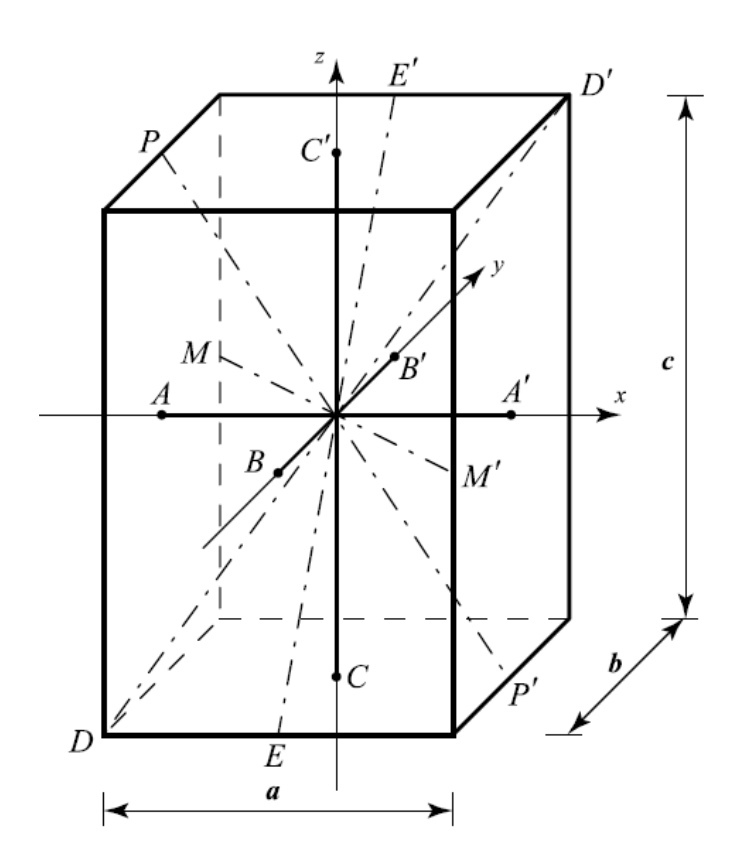
\includegraphics[width=9cm, height=8cm]{parped.jpeg}
\end{center}

\begin{flushright}
{\scriptsize \textbf{Рис 1.} \textbf {Главные оси параллепипеда.}}
\end{flushright}

\begin{center}
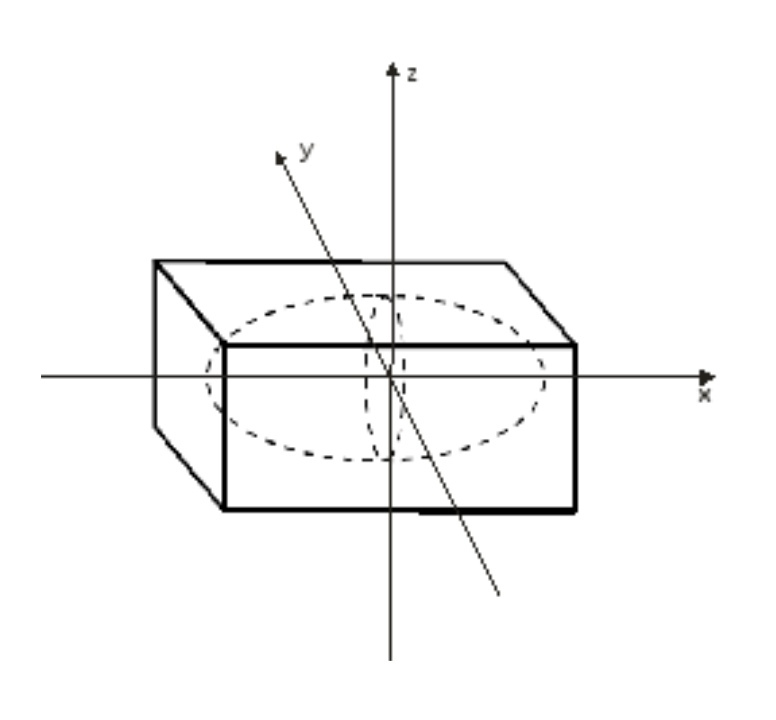
\includegraphics[width=9cm, height=8cm]{iner_parped.jpeg}
\end{center}

\begin{flushright}
{\scriptsize \textbf{Рис 2.1.} \textbf {Эллипсоиды инерции для параллепипеда.}}
\end{flushright}    

\begin{center}
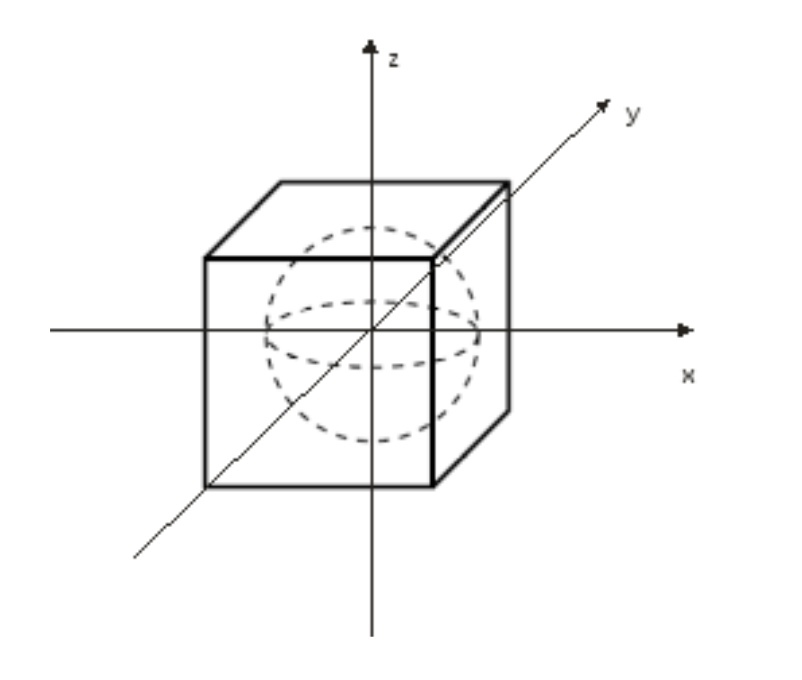
\includegraphics[width=9cm, height=8cm]{iner_cube.jpeg}
\end{center}

\begin{flushright}
{\scriptsize \textbf{Рис 2.2.} \textbf {Эллипсоиды инерции для куба.}}
\end{flushright}

%///////////////////////////////////////////////////////////////////////////////

\section*{3. Оборудование и экспериментальные погрешности}

\subsection*{3.1. Экспериментальная установка}

    В данной работе исползуется рамка крутильных колебаний (см рис.3). В рамке, жёстко закрепленной на проволоке, которая при помощи специальных зажимов может закручиваться и совершать крутильные колебания вдоль вертикальной оси, при помощи планки и гаек закрепляется тело так, чтобы оно было неподвижно во время колебаний самой рамки.
    
\begin{center}
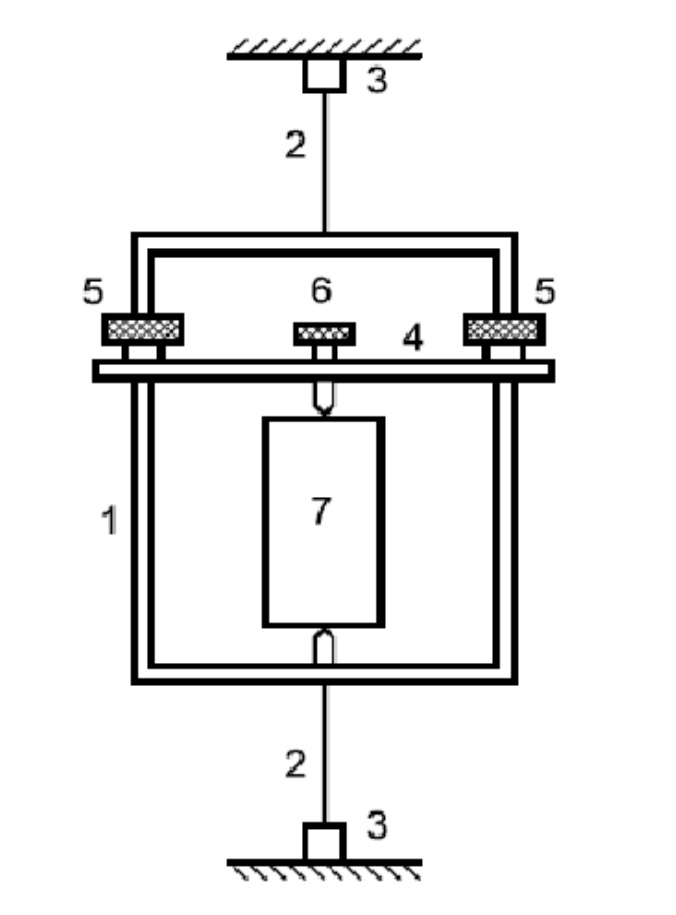
\includegraphics[width=7cm, height=10cm]{ustanovka.jpeg}
\end{center}

\begin{flushright}
{\scriptsize \textbf{Рис 3.} \textbf {Схема экспериментальной установки.}}
\end{flushright}

\subsection*{3.2. Погрешности измерений}

    В данной работе мы пользовались: 
    секундомером для определения времени совершения колебаний рамкой, 
    весами для измерения массы куба, параллелепипеда и диска
    металической линейкой
    штанген-циркулем для измерения размера тел.
    
    
    Соответствующие систематические погрешности приборов:
    
\[\sigma_{t} = 0.01 c\]
\[\sigma_{m} = 0.01 g\]
\[\sigma_{l} = 0.5 mm\]
\[\sigma_{sh} = 0.1 mm\]

    Результаты данных измерений:
    
    для параллелепипеда:
    
\[m = 2083.5 \pm 0.01 g  (\varepsilon = 0.0005 \% \approx 0\%)\]
\[a = 50 \pm 0.5 mm  (\varepsilon = 1 \%)\]
\[b = 100 \pm 0.5 mm  (\varepsilon = 0.5 \%)\]
\[c = 150 \pm 0.5 mm  (\varepsilon = 0.3 \%)\]

    для куба:

\[m = 1089.7 \pm 0.01 g  (\varepsilon = 0.001 \% \approx 0 \%)\]
\[a = b = c = 93 \pm 0.5 mm  (\varepsilon = 0.5\%)\]

    для диска:

\[m = 1569.6 \pm 0.01 g     (\varepsilon = 0.0006 \% \approx 0 \%)\]
\[a = b = 124.6 \pm 0.1 mm  (\varepsilon = 0.08 \%)\]
\[c = 17.1 \pm 0.1 mm  (\varepsilon = 0.5 \%)\]



\section*{4. Результаты измерений и обработка данных}

    Проведём пробный эксперимент с крутильными колебаниями одной рамки без тел для нахождения погрешности и определения периода крутильных колебаний.
    
\begin{table}[h!]
\centering
\begin{tabular}{|l|l|l|}
\hline
N & n  & t     \\ \hline
1 & 10 & 24.53 \\ \hline
2 & 10 & 24.25 \\ \hline
\end{tabular}
\begin{flushright}
{\scriptsize \textbf{Таблица 1.1.} \textbf {Результаты измерений для колебаний рамки без грузов.}}
\end{flushright}
\end{table}


\begin{table}[H]
\centering
\begin{tabular}{|l|l|l|l|}
\hline
Ось & N, раз & t, c  & T, c  \\ \hline
D1B & 10     & 33,94 & 3,394 \\ \hline
D1B & 10     & 33,94 & 3,394 \\ \hline
D1B & 10     & 33,69 & 3,369 \\ \hline
D1B & 10     & 33,84 & 3,384 \\ \hline
D1B & 10     & 33,75 & 3,375 \\ \hline
D1B & 10     & 34,06 & 3,406 \\ \hline
\end{tabular}
\begin{flushright}
{\scriptsize \textbf{Таблица 1.2.} \textbf {Результаты пробного эксперимента для определения случайной погрешности.}}
\end{flushright}
\end{table}


    Случайная погрешность измерения вычисляется по формуле:
    
\[\sigma_{occ} = \sqrt{\frac{1}{N}\sum(T - <\overline{T}>)^2} = 0 С\]

    Полученные данные удивительно точны, так как сумма со значениями периодов равна 0. Это значит, что влияние случайной погрешности на значения данных экспериманта можно не учитывать. Тогда итоговая погрешность измерения периода зависит только от систематической погрешности секундомера $0.01$ с.
    
    
    Период колебаний пустой рамки: 
    
\[T_{p} = 2,439 \pm 0,01 c\]

    Приведём результаты измерений для параллелепипеда, куба и диска в таблицах 2, 3 и 4 соответственно. Количество колебаний n для каждого измерения = 10.Величину $\frac{1}{\sqrt{T^2 - T_p^2}}$ обозначим за $ro$ - она пропорциональна расстоянию от центра масс тела до точки пересечения эллипсоида инерции с соответствующей осью.\\\\\\\\\\\\\\\\\\\\\\\\\
    
    


\begin{table}[H]
\centering
\begin{tabular}{|l|l|l|l|l|}
\hline
Ось  & N, раз & t, c  & T, c  & ro, 1/c \\ \hline
X    & 10     & 40,22 & 4,022 & 0,09777 \\ \hline
X    & 10     & 32,94 & 3,294 & 0,20401 \\ \hline
X    & 10     & 31,72 & 3,172 & 0,24314 \\ \hline
Z    & 10     & 37    & 3,7   & 0,12918 \\ \hline
Z    & 10     & 36,75 & 3,675 & 0,13233 \\ \hline
Y    & 10     & 31,34 & 3,134 & 0,25818 \\ \hline
Y    & 10     & 31,65 & 3,165 & 0,24579 \\ \hline
K1K3 & 10     & 34,32 & 3,432 & 0,17153 \\ \hline
K2K4 & 10     & 34,66 & 3,466 & 0,16490 \\ \hline
M1M3 & 10     & 33,41 & 3,341 & 0,19181 \\ \hline
M2M4 & 10     & 33,53 & 3,353 & 0,18890 \\ \hline
P1P4 & 10     & 32,72 & 3,272 & 0,21020 \\ \hline
P2P5 & 10     & 32,63 & 3,263 & 0,21284 \\ \hline
A1C  & 10     & 33,72 & 3,372 & 0,18445 \\ \hline
B1D  & 10     & 33,97 & 3,397 & 0,17886 \\ \hline
C1A  & 10     & 34,04 & 3,404 & 0,17735 \\ \hline
D1B  & 10     & 33,87 & 3,387 & 0,18106 \\ \hline
\end{tabular}
\begin{flushright}
{\scriptsize \textbf{Таблица 2.} \textbf {Результаты измерений для параллелепипеда.}}
\end{flushright}
\end{table}



\begin{table}[H]
\centering
\begin{tabular}{|l|l|l|l|l|}
\hline
Ось  & N, раз & t, c  & T, c  & ro, 1/c \\ \hline
X    & 10     & 30,31 & 3,031 & 0,3088  \\ \hline
Y    & 10     & 30,12 & 3,012 & 0,3202  \\ \hline
Z    & 10     & 30,22 & 3,022 & 0,3141  \\ \hline
M1M3 & 10     & 30,35 & 3,035 & 0,3065  \\ \hline
M2M4 & 10     & 30,06 & 3,006 & 0,3239  \\ \hline
K1K3 & 10     & 30,37 & 3,037 & 0,3054  \\ \hline
K2K4 & 10     & 30,35 & 3,035 & 0,3065  \\ \hline
AC1  & 10     & 30,53 & 3,053 & 0,2966  \\ \hline
B1D  & 10     & 30,37 & 3,037 & 0,3054  \\ \hline
CA1  & 10     & 30,34 & 3,034 & 0,3071  \\ \hline
BD1  & 10     & 30,88 & 3,088 & 0,2788  \\ \hline
P1P4 & 10     & 30,38 & 3,038 & 0,3048  \\ \hline
P2P5 & 10     & 30,41 & 3,041 & 0,3031  \\ \hline
\end{tabular}
\begin{flushright}
{\scriptsize \textbf{Таблица 3.} \textbf {Результаты измерений для куба.}}
\end{flushright}    
\end{table}

\begin{table}[H]
\centering
\begin{tabular}{|l|l|l|l|l|}
\hline
Ось & N, раз & t, c  & T, c  & ro, 1/c \\ \hline
X   & 10     & 30    & 3     & 0,3277  \\ \hline
X   & 10     & 30,16 & 3,016 & 0,3177  \\ \hline
Z   & 10     & 34    & 3,4   & 0,1782  \\ \hline
Z   & 10     & 33,97 & 3,397 & 0,1789  \\ \hline
\end{tabular}
\begin{flushright}
{\scriptsize \textbf{Таблица 4.} \textbf {Результаты измерений для диска.}}
\end{flushright}
\end{table}

\subsection*{4.1. Проверка теоретических предположений}

    На основе полученных данных проверим правильность следующих формул:
    
\[(a^2+b^2+c^2)T_d^2 = a^2T_x^2 + b^2T_y^2 + c^2T_z^2\]
\[(b^2+c^2)T_E^2 = b^2T_y^2 + c^2T_z^2\]
\[(a^2+c^2)T_P^2 = a^2T_x^2 + c^2T_z^2\]
\[(a^2+b^2)T_M^2 = a^2T_x^2 + b^2T_y^2\]

    Рассчитаем погрешности полученных величин:
    
\[f = (a^2 + b^2 + c^2)T^2\]
\[\sigma_p^2 = \left(\frac{df}{da}\right)\sigma_a^2 + \left(\frac{df}{db}\right)\sigma_b^2 + \left(\frac{df}{dc}\right)\sigma_c^2 + \left(\frac{df}{dT}\right)\sigma_T^2 =\]
\[= (2aT^2)^2\sigma_a^2 +(2bT^2)^2\sigma_b^2 +(2cT^2)^2\sigma_c^2 + (2(a^2 + b^2 + c^2)T)^2\sigma_T^2\]

\[\sigma_p = 0,014 m^2c^2\]

\[\sigma_k = 0,01 m^2c^2\]


    Полученные формулы для параллелепипеда:
\[ 0,4311 \pm 0,014 = 0,4313 \pm 0,014\]
\[ 0,3904 \pm 0,014 = 0,4051 \pm 0,014\]
\[ 0,3041 \pm 0,014 = 0,3321 \pm 0,014\]
\[ 0,1331 \pm 0,014 = 0,1284 \pm 0,014\]
    
    
    для куба:
\[ 0,2474 \pm 0,01 = 0,2369 \pm 0,01\]
\[ 0,1595 \pm 0,01 = 0,1575 \pm 0,01\]
\[ 0,1593 \pm 0,01 = 0,1584 \pm 0,01\]
\[ 0,1600 \pm 0,01 = 0,1579 \pm 0,01\]




    Все эти равентва выполняются в пределах 3 $\sigma$.Следовательно, теоретические предположения подтвердились на практике и оказались верны.

\subsection*{4.2. Построение эллипсоидов инерции}

    По вычисленным величинам $ro = \frac{1}{\sqrt{T^2 - T_p^2}}$ построим сечения  эллипсоидов энерции для параллелепипеда (по 3 главным плоскостям), куба (по одной - тк по всем плоскостям получается такая же окружность) и диска (по одной - остальные аналогичны) (см. рис. 4).

\begin{center}
    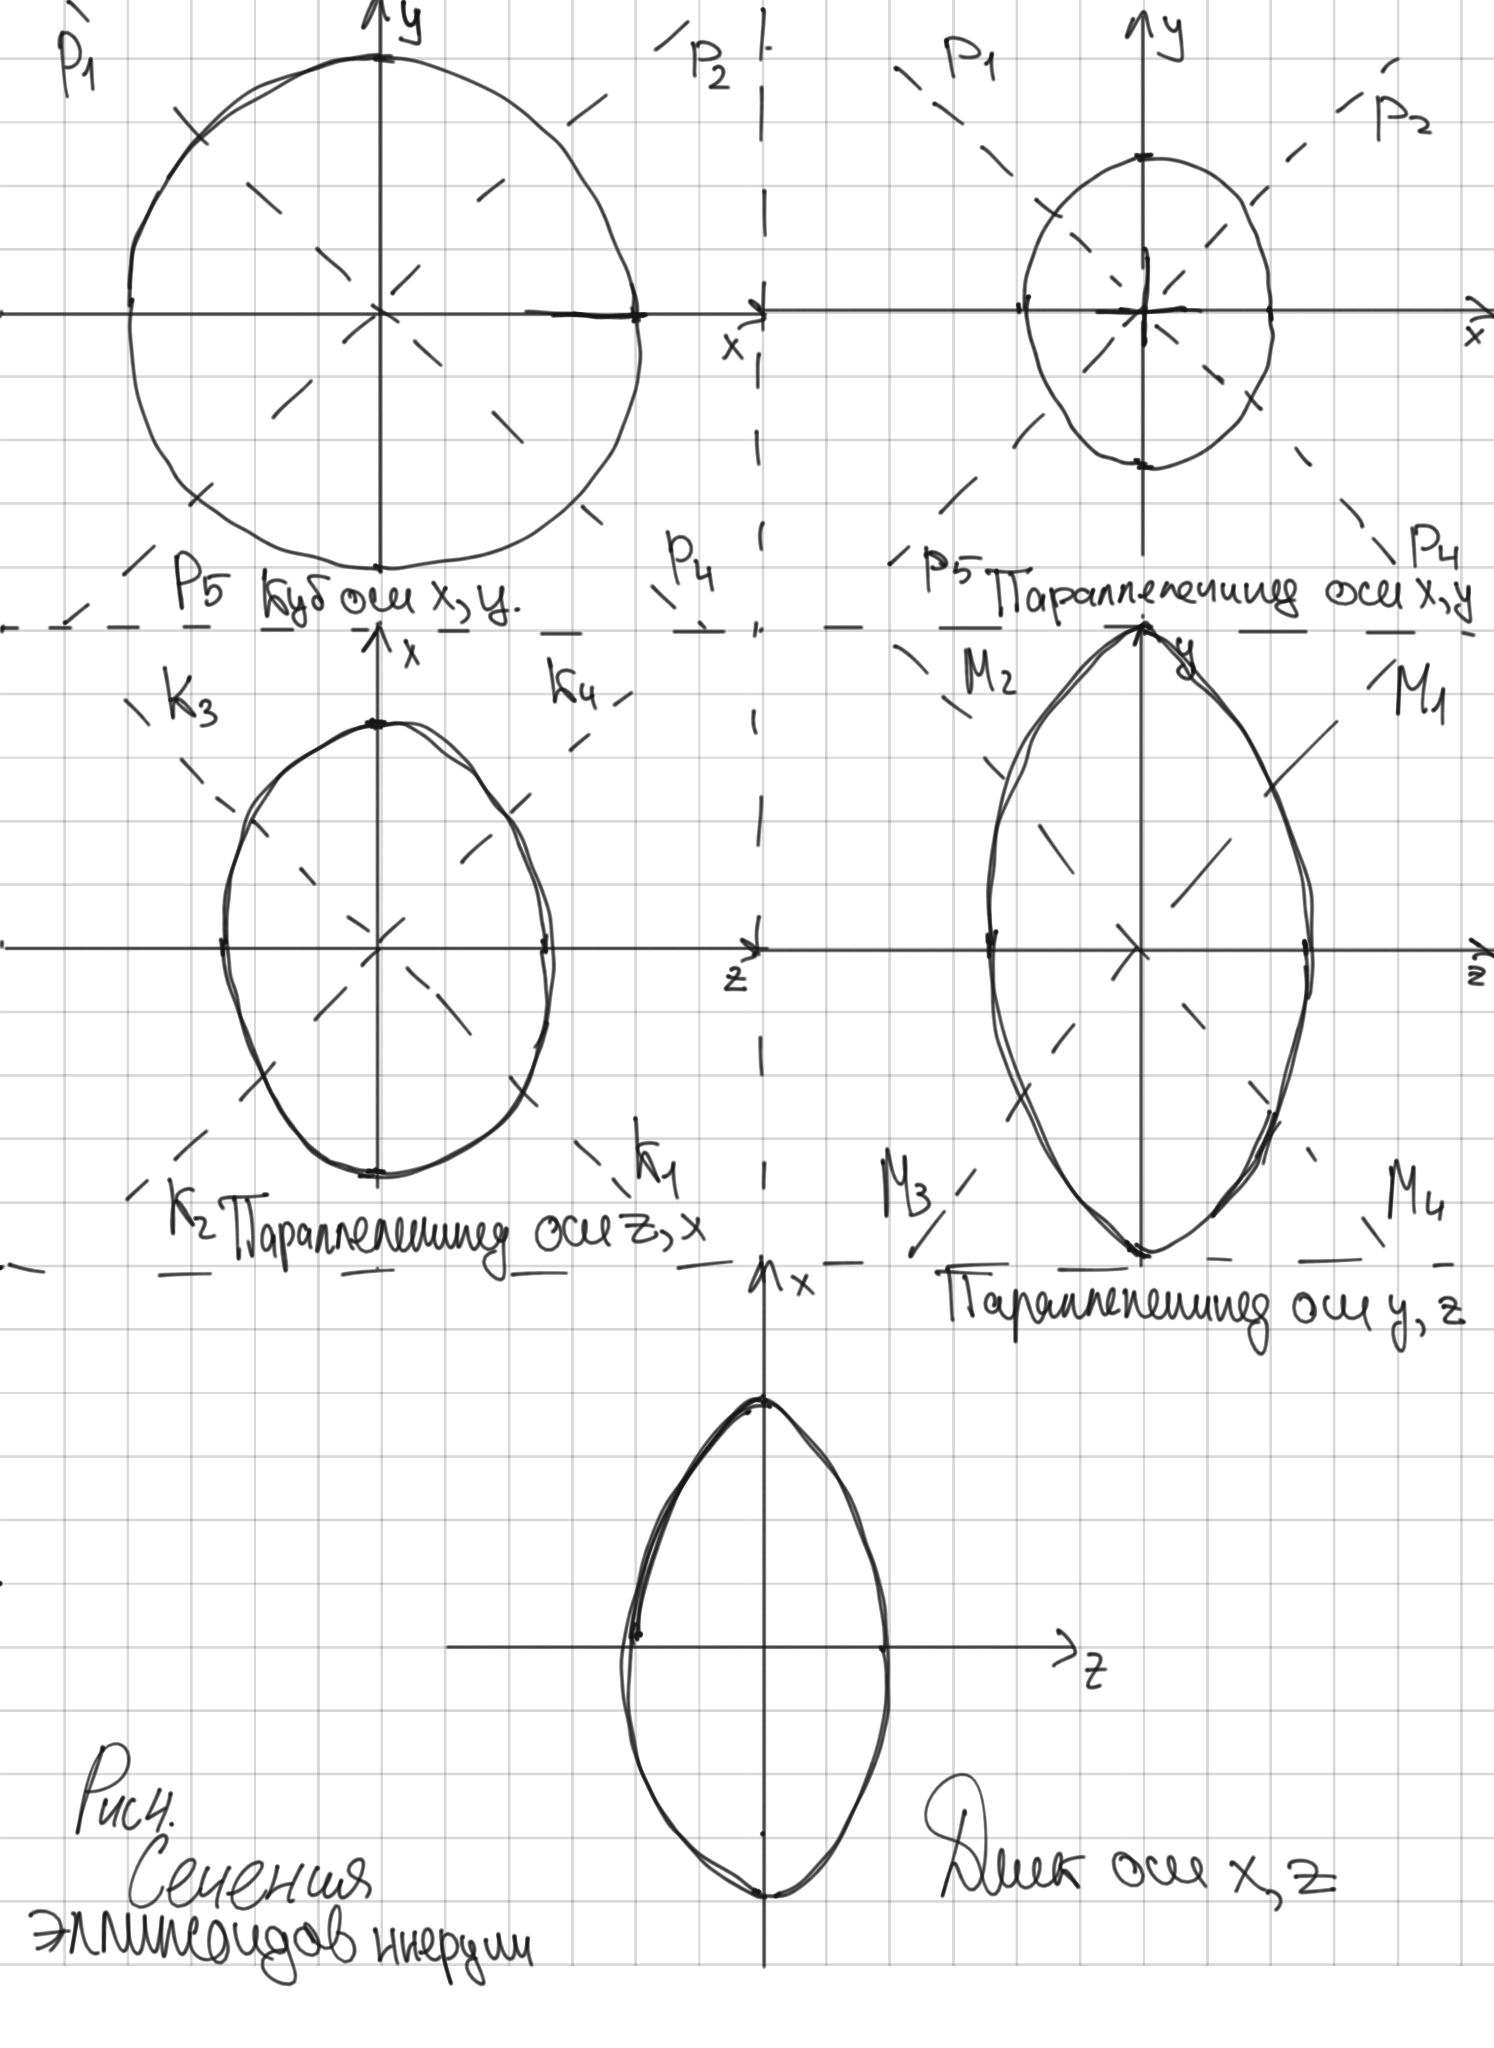
\includegraphics[scale = 0.2]{ell.png}
\end{center}

\begin{flushright}
{\scriptsize \textbf{Рис 4.} \textbf {Сечения эллипсоидов энерции для параллелипипеда, куба и диска.}}
\end{flushright}
    

\section*{5. Обсуждение результатов и выводы}

    В ходе работы мы проверили верность формул зависимости периодов крутильных колебаний 2 твердых тел (параллелепипеда и куба), а также по полученным в ходе эксперимента данным построили сечения эллипсоидов инерции для них же и диска.
    


%/////////////////////////////////////////////////////////////////////////
\end{document}
